%\RequirePackage[]{optional}
%\RequirePackage[slides]{optional}
\RequirePackage[notslides]{optional}

\opt{slides}{
% Following for presentation mode
\documentclass[10pt]{beamer}
\usepackage{xmpmulti}
%usetheme{Berlin}
}
\opt{notslides}{
% Following for notes mode
\documentclass[a4paper]{article}
\usepackage{beamerarticle}
\usepackage{a4wide}
\usepackage{graphicx}
\usepackage{amsfonts}
\usepackage{fancyhdr}
}

% Following for all modes
%\usepackage{auto-pst-pdf}
%\usepackage{pst-pdf}
\usepackage{psfrag}
\usepackage{setspace}

\parindent=0ex
\parskip=1ex
\newcommand{\conv}{\ast}
\newcommand{\ftpair}{{\stackrel{\cal F}{\longleftrightarrow}}}
\reversemarginpar

%\title{Fourier transform}
%\author{}
%\date{}

\begin{document}
\pagestyle{fancy}
\fancyhead{}
\renewcommand{\headrulewidth}{0pt}
\fancyfoot[C]{\thesection-\thepage}
%\fancyfoot[R]{fcn2010}

\begin{frame}
\titlepage
\end{frame}

\setcounter{section}{5}
\section{Filtering}

A complete description of a LTI system is shown below:
\begin{center}
  \psfrag{x(t)}{\scriptsize $x(t)$}
  \psfrag{y(t)}{\scriptsize $y(t) = h(t) \conv x(t)$}
  \psfrag{h(t)}{\scriptsize $h(t)$}
  \psfrag{X(w)}{\scriptsize $X(\omega)$}
  \psfrag{Y(w)}{\scriptsize $Y(\omega) = H(\omega) X(\omega)$}
  \psfrag{H(w)}{\scriptsize $H(\omega)$}
  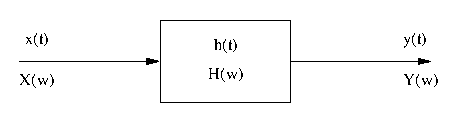
\includegraphics{simpleltisystemtf}
\end{center}
On the top is a time-domain description, in terms of time-domain signals, the system impulse response $h(t)$, and the convolution operation for finding the system output.  On the bottom is the frequency-domain description, using frequency-domain descriptions of signals, the {\em frequency response} or {\em transfer function} $H(\omega)$, and multiplication for finding the system output.  Given the impulse response we can find the frequency response, and vice versa:  the two descriptions are entirely equivalent.  However, since multiplication is a simpler operation to understand than convolution, the second description is more intuitive and we prefer it.

A main applications of LTI systems is to perform filtering.  A system takes an input signal.  It produces an output signal that is related to the input, according to the system properties.  In practice we can define systems that have desirable properties, and these systems take input signals and produce output signals that are useful for our purposes.

Most of the time we specify the properties we require from a system in the frequency domain.  This involves specifying $H(\omega)$.  In effect, we {\em design} a system that has a frequency response that approximates the requirements for our application.

\subsection{Ideal lowpass filter}

Applying the duality property to the Fourier pair
\begin{equation*}
  p_{\tau}(t) \quad \ftpair \quad \tau \text{sinc} \left( \frac{\tau \omega}{2 \pi} \right)
\end{equation*}
gives the new pair
\begin{equation*}
  \tau \text{sinc} \left( \frac{\tau t}{2 \pi} \right) \quad \ftpair \quad 2 \pi p_{\tau}(-\omega)
  = 2 \pi p_{\tau}(\omega),
\end{equation*}
since $p_{\tau}(\omega) = p_{\tau}(-\omega)$ is an even function.  By linearity,
\begin{equation*}
  \frac{\tau}{2 \pi} \text{sinc} \left( \frac{\tau t}{2 \pi} \right) \quad \ftpair \quad p_{\tau}(\omega).
\end{equation*}
A $\text{sinc}$ in the time domain transforms to a rectangular pulse in frequency.  

Now consider the system
\begin{center}
  \psfrag{x(t)}{\scriptsize $x(t)$}
  \psfrag{y(t)}{\scriptsize $y(t)$}
  \psfrag{h(t)}{\scriptsize $h(t)$}
  \psfrag{X(w)}{\scriptsize $X(\omega)$}
  \psfrag{Y(w)}{\scriptsize $Y(\omega)$}
  \psfrag{H(w)}{\scriptsize $H(\omega)$}
  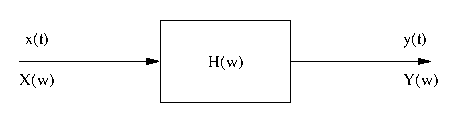
\includegraphics{simpleltisystemfreq}
\end{center}
with $H(\omega) = p_2(\omega)$.  The frequency response is the real-valued function below:
\begin{center}
  \psfrag{w}{\scriptsize $\omega$}
  \psfrag{H(w)}{\scriptsize $H(\omega)$}
  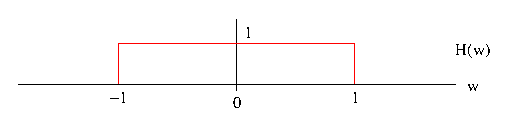
\includegraphics{ideallpffreq}
\end{center}
What is the output of the system when the input is $x(t) = e^{j \omega_0 t}$ for some specific value of $\omega_0$?

The definition of the frequency response provides the most direct way of obtaining the solution.  Recall that for any LTI system the following is a valid input-output pair:
\begin{equation*}
  e^{j \omega_0 t} \quad \longrightarrow \quad H(\omega_0) e^{j \omega_0 t}.
\end{equation*}
The (possibly complex) value $H(\omega_0)$ completely determines the action of the system on a signal at frequency $\omega_0$, or in other words on the signal $e^{j \omega_0 t}$.  Thus the output will be $y(t) = H(\omega_0) e^{j \omega_0 t}$.  Looking at the transfer function $H(\omega)$ above we see that the output will depend on the value of $\omega_0$:
\begin{equation*}
  y(t) = \begin{cases}
    e^{j \omega_0 t} \qquad & -1 \leq \omega_0 \leq 1 \\
    0 \qquad & \text{otherwise}.
  \end{cases}
\end{equation*}
If the frequency of the input complex exponential is in the passband of the filter, that is if $|\omega| \leq 1$, then it propagates through without modification.  The system passes low frequencies.  However, if the input is a complex exponential with a frequency $|\omega_0| > 1$, then the output is zero:  the system completely blocks signals at high frequencies.   The system is therefore a lowpass filter.  It passes low frequency signals without modification, and eliminates high frequencies.  Also, the system is ideal because the transition between the passband $|\omega| \leq 1$ and the stopband $|\omega|>1$ is infinitely sharp.

Another way of looking at this scenario is to simply use frequency-domain reasoning.  The input signal $x(t) = e^{j \omega_0 t}$ has a frequency representation $X(\omega) = 2 \pi \delta(\omega - \omega_0)$, which consists of exactly one impulse at $\omega = \omega_0$.  The output of the filter is the product $Y(\omega) = H(\omega) X(\omega)$.  If the impulse lies in the passband $|\omega| \leq 1$ of the filter (that is, if $|\omega_0| \leq 1$), then the output is $Y(\omega) = 2 \pi \delta(\omega - \omega_0)$.  The time-domain output in this case is just $y(t) = e^{j \omega_0 t}$, the same as the input.  However, if $|\omega_0| > 1$ then $Y(\omega) = 0$, so $y(t) = 0$.  

Since the ideal lowpass filter is LTI (otherwise the frequency response $H(\omega)$ would not exist), it has an equivalent description in terms of an impulse response.  The impulse response in this case is
\begin{equation*}
  h(t) = \frac{2}{2 \pi} \text{sinc} \left( \frac{2 t}{2 \pi} \right),
\end{equation*}
which has the form of a $\sin(x)/x$ function in time.  Since the system is governed by the covolution $y(t) = h(t) \conv x(t)$, we see that an ideal lowpass filter convolves the time-domain input $x(t)$ with a $\text{sinc}$ function to obtain the output.  The output for $x(t) = e^{j \omega_0 t}$ will be
\begin{equation*}
  y(t) = \frac{1}{\pi} \text{sinc} \left( \frac{t}{\pi} \right) \conv e^{j \omega_0 t}.
\end{equation*}
The result of this convolution is $e^{j \omega_0 t}$ if $|\omega| \leq 1$ and zero if $|\omega_0| > 1$.  This is obvious from frequency-domain reasoning, but completely non-intuitive in the time domain.

\subsection{RC lowpass filter}

An ideal lowpass filter is conceptually useful, but we can't build one in practice.  Because the impulse response is infinitely long (there is no point in time beyond which it is always equal to zero) we need to know the input $x(t)$ for {\it all} time to calculate the output $y(t)$ at any single instant --- and we can never measure a signal for all time.  Also, note that the $\sin(x)/x$ impulse response is not zero for negative time (that is, it is not right-sided), so the ideal lowpass filter is not causal.  This can be a problem if we want to filter a signal online in real time, which is often required.  Nonetheless, we often try to design systems that at least approximate the ideal lowpass filter frequency response.

The simplest electrical system that we can construct to approximate a lowpass filter is the RC circuit shown below:
\begin{center}
  \psfrag{x(t)=v(t)}{\scriptsize $x(t)=v(t)$}
  \psfrag{vC(t)=y(t)}{\scriptsize $v_C(t)=y(t)$}
  \psfrag{vR(t)}{\scriptsize $v_R(t)$}
  \psfrag{i(t)}{\scriptsize $i(t)$}
  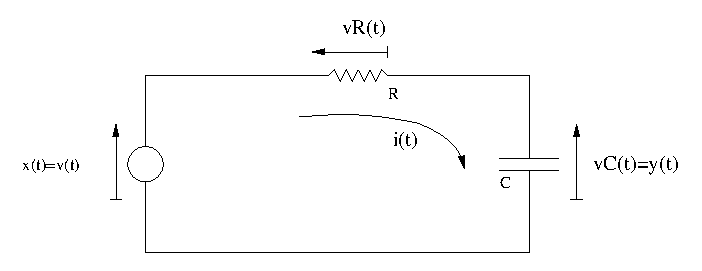
\includegraphics{circuitrclowpass}
\end{center}
The input is the voltage generated by the voltage source on the left, and the output is the voltage across the capacitor on the right.

We know the time-domain models that govern the behaviour of resistors and capacitors, so we can find a differential equation relating the input $x(t)$ to the output $y(t)$.  The fundamental relationship defining a resistor is $V/I=R$.  However, this is only for constant $V$ and $I$ --- the whole point of signal analysis is to reason about quantities that vary with time.  If $R$ is constant but the voltage and current can vary, then the usual equation generalises to $v(t)/i(t) = R$, or $v(t) = R i(t)$.  This relationship must hold for all $t$ in the model of a resistor:  the voltage across it must always equal $R$ times the current through it at any instant in time.  In the diagram above the voltage across the resistor is denoted by $v_R(t)$, so the governing equation in terms of the signals shown is $v_r(t) = R i(t)$.

Similarly we consider the voltage across the capacitor to be a function $v_C(t)$ of time.  Using the principles of electrostatics one finds the time-domain relationship linking the voltage $v_C(t)$ across a capacitor and the current $i(t)$ through it to be $i(t) = C \frac{dv_C(t)}{dt}$, where $C$ is defined to be the capacitance.  Unlike the resistor the equations governing a capacitor {\em have} to be specified in terms of functions of time, since it is a dynamic device.

The last equation that is required to specify the input-output relation involves potentials.  If we consider the bottom wire of the circuit to be ground, then the potential above the voltage source is $v(t)$.  However, this potential must be equal to the sum of the voltages across the resistor and the capacitor (properly directed as shown), so $v(t) = v_C(t) + v_R(t)$.  This must also hold for all instants in time.

The three equations that determine the behaviour of the circuit are therefore
\begin{equation*}
  v_R(t) = R i(t), \qquad i(t) = C \frac{dv_C(t)}{dt}, \qquad \text{and} \qquad v(t) = v_C(t) + v_R(t).
\end{equation*}
Eliminating $v_R(t)$ from the first and third equations gives
\begin{equation*}
  \qquad i(t) = C \frac{dv_C(t)}{dt} \qquad \text{and} \qquad v(t) = v_C(t) + R i(t),
\end{equation*}
and now eliminating $i(t)$ gives
\begin{equation*}
  v(t) = v_C(t) + R C \frac{dv_C(t)}{dt}.
\end{equation*}
Finally, noting that the input is defined to be $x(t) = v(t)$ and the output $v_C(t) = y(t)$ gives the overall input-output relationship:
\begin{equation*}
  x(t) = y(t) + R C \frac{dy(t)}{dt}.
\end{equation*}
For any given input $x(t)$ one can in principle solve this differential equation for $y(t)$, so we now have an input-output relation for the system.

Resistors and capacitors (and inductors) are linear and time-invariant devices, so any system constructed from these passive devices is LTI.  (Transistors, on the other hand, are active devices that are often operated in a nonlinear region.)  The RC circuit therefore has an impuse response $h(t)$, which could be found by calculating the output $y(t)$ when the input is $x(t) = \delta(t)$.  That is, the impulse response $h(t)$ must satisfy $\delta(t) = h(t) + RC \frac{dh(t)}{dt}$.  This equation is not easy to solve.

Fourier methods present a way forward.  Since the system is LTI it has a frequency response $H(\omega)$ that equals the Fourier transform of $h(t)$.  Now, if we take the Fourier transform of both sides of the expression $\delta(t) = h(t) + RC \frac{dh(t)}{dt}$ we get
\begin{equation*}
  1 = H(\omega) + RC j \omega H(\omega),
\end{equation*}
which is an algebraic equation rather than a differential equation.  We can factorise it as $1 = H(\omega)(1 + j \omega RC)$, and solve for $H(\omega)$:
\begin{equation*}
  H(\omega) = \frac{1}{1 + j \omega RC} = \frac{\frac{1}{RC}}{\frac{1}{RC} + j \omega}.
\end{equation*}
The inverse transform then yields the impulse response
\begin{equation*}
  h(t) = \frac{1}{RC} e^{-\frac{1}{RC} t} u(t),
\end{equation*}
which is plotted below:
\begin{center}
  \psfrag{t}{\scriptsize $t$}
  \psfrag{h(t)}{\scriptsize $h(t)$}
  \psfrag{1/RC}{\scriptsize $\frac{1}{RC}$}
  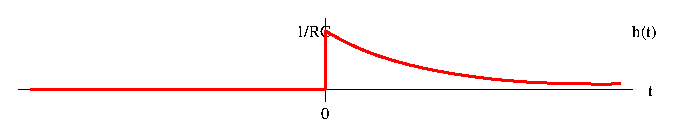
\includegraphics{circuitrclpir}
\end{center}
Mathematically, the RC lowpass filter given takes the input $x(t)$ and convolves it with this function to give the output $y(t)$.  The quantity $\tau = RC$ is called the {\em time constant} of the circuit, and can quite easily be shown to be the time required for the impulse response voltage to fall to $1/e$ of its initial value.  

Recall that the impulse response is the output of the circuit when the input is $\delta(t)$.  While we can't actually generate a delta function, and therefore can't put one into a real circuit, we certainly {\em can} put one into a mathematical model of our circuit.  The interpretation is as follows.  Initially there is zero voltage at the input and the circuit is at rest --- the capacitor is discharged and the output voltage is zero.  At time $t=0$ the circuit is "kicked" by an impulse, which instantaneously transfers a charge to the capacitor.  The output voltage immediately jumps to $\frac{1}{RC}$.  After this time the input voltage returns to zero, so the voltage source is effectively a short circuit.  The capacitor discharges through the resistor, so the output voltage gradually drops.  If $R$ is big then the discharge is slow, so the impulse response falls off gradually.  Similarly, if the capacitor is big then the discharging is also slow.  The product $\tau = RC$ is a parameter that takes both of these effects into accout:  when large the rate of decay of $h(t)$ is low, and when small it is high.  

If one doesn't explicitly need the impulse response or the frequency response then the original differential equation linking input and output can be used directly:  the equation $x(t) = y(t) + R C \frac{dy(t)}{dt}$ can be Fourier transformed to give an input-output relation in the frequency domain:
\begin{equation*}
  X(\omega) = Y(\omega) + RC j \omega Y(\omega) = Y(\omega) (1 + j \omega RC).
\end{equation*}
We can express any input $x(t)$ in terms of its Fourier transform $X(\omega)$, in which case the Fourier transform of the output is
\begin{equation*}
  Y(\omega) = \frac{1}{1 + j \omega RC} X(\omega).
\end{equation*}
Note that this is just a statement of the expression $Y(\omega) = H(\omega) X(\omega)$, which is the frequency-domain counterpart of the time-domain input-output relationship defined by convolution:  $y(t) = h(t) \conv x(t)$.

\subsection{Frequency-domain analysis of RC lowpass filter}

We normally visualise filters (and signals) in the frequency domain.  We showed that the RC lowpass filter in the previous section has a transfer function or frequency response of
\begin{equation*}
  H(\omega) = \frac{1}{1 + j \omega RC}.
\end{equation*}
To understand this filter it helps to plot the transfer function --- both magnitude and phase, since it is generally complex.  To express this transfer function in polar coordinates we consider ${1 + j \omega RC}$.  For each value of $\omega$ this is a point in the Argand diagram,
[draw]
and by consdiering the length and angle of this vector we see that it can be written as
\begin{equation*}
  1 + j \omega RC = \sqrt{1 + \omega^2 (RC)^2} e^{j \arctan(\omega RC)},
\end{equation*}
The required frequency response is therefore
\begin{equation*}
  H(\omega) = \frac{1}{1 + j \omega RC} = \frac{1}{\sqrt{1 + \omega^2 (RC)^2}} e^{-j \arctan(\omega RC)},
\end{equation*}
which is plotted below for $R = C = 1$:
\begin{center}
  \psfrag{|H(w)|}{\scriptsize $|H(\omega)|$}
  \psfrag{aH(w)}{\scriptsize $\angle H(\omega)$}
  \psfrag{pi}{\scriptsize $\pi$}
  \psfrag{2*pi}{\scriptsize $2\pi$}
  \psfrag{-pi}{\scriptsize $-\pi$}
  \psfrag{-2*pi}{\scriptsize $-2\pi$}
  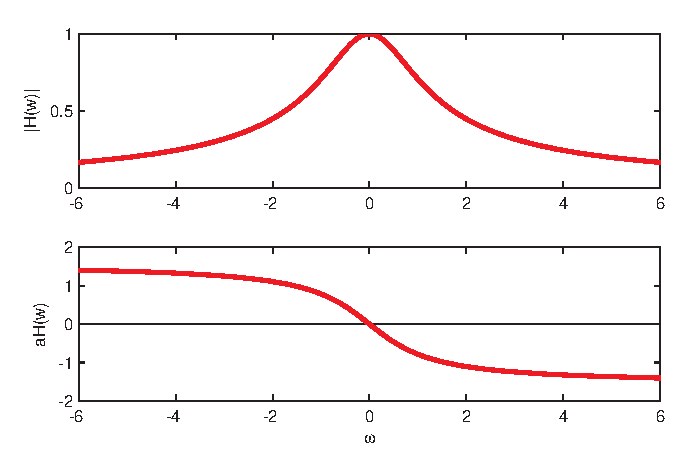
\includegraphics{circrclptf}
\end{center}
This is called the {\em Bode plot} of the system (although typically Bode plots are displayed on logarithmic axes, as will be shown shortly).  

The definition of the frequency response states that an input of $x(t) = e^{j \omega_0 t}$ to the system produces an output $y(t) = H(\omega_0) e^{j \omega_0 t}$.  Therefore an input of $x(t) = e^{j 2 t}$ will produce the output
\begin{align*}
  y(t) &= H(2) e^{j 2 t} = \frac{1}{\sqrt{1 + 2^2 (RC)^2}} e^{-j \arctan(2 RC)} e^{j 2 t} \\
  & = \frac{1}{\sqrt{1 + 2^2 (RC)^2}} e^{j( 2t - \arctan(2 RC))}
  = |H(2)| e^{j (2t + \angle H(2))},
\end{align*}
which for the $R = C = 1$ case plotted above gives
\begin{equation*}
  y(t) = 0.4472 e^{j (2t - 1.1071)}.
\end{equation*}
Note that the values in this result can be read directly off of the graph at $\omega = 2$.  Thus the plot of the frequency response immediately carries all of the useful information about what happens to any given frequency at the input as it passes through the system.  We see that this RC lowpass filter tends to reduce the magnitude of high frequencies:  the effectively get multiplied by a number with a small magnitude, and their amplitude decreases accordingly.  

The magnitude $|H(\omega)|$ of the frequency response is called the {\em gain} of the system for frequency $\omega$.  If the gain is greater than one then the amplitude of a complex exponential input at that frequency will be amplified by the corresponding gain value; otherwise it will be reduced.  However, engineers and physicists often prefer to express the gain on a logarithmic scale, also called the decibel (dB) scale, which for a voltage signal is defined as
\begin{equation*}
  G_{\text{dB}}(\omega) = 20 \log_{10} |H(\omega)|.
\end{equation*}
To investigate this further we define $\omega_c = 1/\tau = \frac{1}{RC}$, and from the magnitude response calculated earlier for the RC lowpass system we see that
\begin{align*}
  G_{\text{dB}}(\omega) &= 20 \log_{10} \frac{1}{\sqrt{1 + (\omega RC)^2})}
  = 20 \log_{10} \frac{1}{\sqrt{1 + (\omega/\omega_c)^2})} \\
  &= 20 \log_{10} (\sqrt{1 + (\omega/\omega_c)^2})^{-1} 
  = -20 \log_{10} (\sqrt{1 + (\omega/\omega_c)^2})
\end{align*}
A plot of the gain in dB versus frequency on a log axis for the case of $\omega_c = 1$ is shown as the solid (red) curve below:
\begin{center}
  \psfrag{w}{\scriptsize $\omega$}
  \psfrag{Gain GdB(w)}{\scriptsize Gain $G_{dB}(\omega)$}
  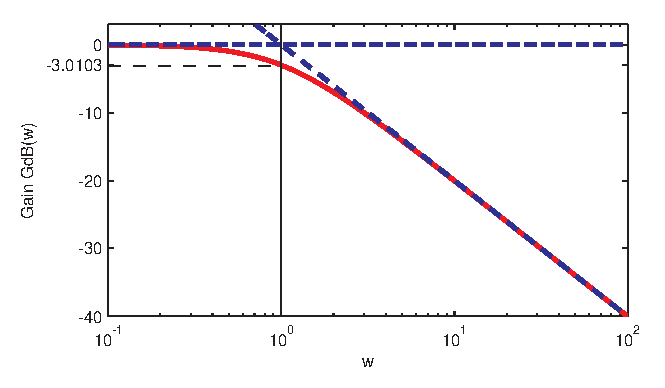
\includegraphics{rclpfbodemag}
\end{center}
Also shown are dotted (blue) asymptotes to the curve.  Firstly, for $\omega \ll \omega_c$ the gain is approximately $G_{\text{dB}}(\omega) \approx -20 \log_{10} (\sqrt{1}) = 0$.  This is the horizontal asymptote in the plot.  Secondly, for $\omega \gg \omega_c$ the ratio $\omega/\omega_c \gg 1$ and $\sqrt{1 + (\omega/\omega_c)^2} \approx \sqrt{(\omega/\omega_c)^2} = \omega/\omega_c$, so the gain is approximately
\begin{equation*}
  G_{\text{dB}}(\omega) \approx -20 \log_{10} (\omega/\omega_c)
  = -20 \log_{10} (\omega) + 20 \log_{10}(\omega_c).
\end{equation*}
This is the asymptote in the plot that matches the curve for high frequencies, and defines what is called the {\em roll-off} of the filter.  We observe that in this region an increase in frequency by a factor of 10 (e.g. from $10^0$ to $10^1$, or from $10^1$ to $10^2$) always reduces the gain by 20dB.  We therefore say that the filter has a roll-off of  20dB/decade, which is a measure of how effectively the lowpass filter attentuates or reduces high frequencies.  Equivalently, it is quite easy to show that when the frequency doubles in this region the gain drops by 6dB.  Since going up an octave corresponds to a doubling of frequency (also in music!), we could equivalently say that the filter has a roll-off of 6dB/octave.  Note that this is the roll-off rate of {\em any} first-order lowpass filter.

The two asymptotes cross at $\omega = \omega_c$, which is called the {\em cut-off}, {\em breakpoint}, or {\em knee} of the filter --- effectively it can be considered the frequency at which the filter transitions from the low-frequency pass band to the high-frequency stop band.  Noting that at this frequency we have $\sqrt{1 + (\omega/\omega_0)^2} = \sqrt{1 + (\omega_0/\omega_0)^2} = \sqrt{2}$, we see that
\begin{equation*}
  G_{\text{dB}}(\omega_0) = -20 \log_{10}(\sqrt{2}) = -3.0103.
\end{equation*}
The cut-off frequency $\omega_c$ of the filter is therefore also called the $-3$dB point.  It can be expressed in Hertz by noting that $\omega_c = 2 \pi f_c$ and $\omega_c = \frac{1}{RC}$, so
\begin{equation*}
  f_c  = \frac{1}{2 \pi RC}.
\end{equation*}
The cut-off frequency of the RC lowpass filter can therefore be varied by changing either $R$ or $C$, and for mathematical purposes only the product $RC$ (equal to the circuit time constant $\tau$) matters.

{\em Repeat\marginpar{\bf Exercise:} the whole analysis for a first-order highpass filter, where the resistor and the capacitor in the circuit are swapped.}

\subsection{Response to a real-valued sinusoid}

The frequency response of an LTI system can easily be used to find the output $y(t)$ when the input is the sinusoidal signal $x(t) = A \cos(\omega_0 t + \phi)$.  The result follows from the input-output pair
\begin{equation*}
  e^{j \omega_0 t} \quad \longrightarrow \quad H(\omega_0) e^{j \omega_0 t}.
\end{equation*}
Since we can write
\begin{equation*}
  x(t) = A/2 e^{j \omega_0 t + \phi} + A/2 e^{-j \omega_0 t + \phi} 
  = (A/2 e^{j \phi}) e^{j \omega_0 t} + (A/2 e^{-j \phi}) e^{-j \omega_0 t} 
\end{equation*}
the required output is
\begin{equation*}
  y(t) = (A/2 e^{j \phi}) H(\omega_0) e^{j \omega_0 t} + (A/2 e^{-j \phi}) H(-\omega_0) e^{-j \omega_0 t}.
\end{equation*}
If the impulse response $h(t)$ is real valued then $H(\omega)$ is conjugate symmetric, so
\begin{equation*}
  H(\omega_0) = |H(\omega_0)| e^{j \angle H(\omega_0)} \qquad \text{and} \quad
  H(-\omega_0) = H^\ast(\omega_0) = |H(\omega_0)| e^{-j \angle H(\omega_0)}.
\end{equation*}
Substituting and rearranging gives the following:
\begin{align*}
  y(t) &=  (A/2 e^{j \phi}) |H(\omega_0)| e^{j \angle H(\omega_0)} e^{j \omega_0 t} 
  + (A/2 e^{-j \phi}) |H(\omega_0)| e^{-j \angle H(\omega_0)} e^{-j \omega_0 t} \\
  &= A/2 |H(\omega_0)| e^{j (\omega_0 t + \phi + \angle H(\omega_0))} +
  A/2 |H(\omega_0)| e^{-j (\omega_0 t + \phi + \angle H(\omega_0))} \\
  &= A |H(\omega_0)| \cos(\omega_0 t + \phi + \angle H(\omega_0)).
\end{align*}
Thus the following input-output pair results:
\begin{equation*}
  A \cos(\omega_0 t + \phi) \quad \longrightarrow \quad A |H(\omega_0)| \cos(\omega_0 t + \phi + \angle H(\omega_0).
\end{equation*}
A sinusoid of frequency $\omega_0$ at the input results in a sinusoid of the same frequency at the output, but with magnitude scaled by the factor $|H(\omega_0)|$ and phase shifted by $\angle H(\omega_0)$.  These two values can be obtained from the complex frequency response $H(\omega)$ evaluated at the frequency $\omega_0$ of the input.

LTI systems do not generate frequencies at the output that are not present at the input.  For AC analysis at a fixed frequency this makes it possible to use {\em phasor notation} to perform the required calculations.  With fixed $\omega_0$ the sinusoidal signal $x(t) = A \cos(\omega_0 t + \phi)$ has two free parameters, $A$ and $\phi$, and we can represent it by the quantity $\tilde{X}$ in the phasor domain:
\begin{equation*}
  x(t) = A \cos(\omega_0 t + \phi) \quad \longrightarrow \quad \tilde{X} = A e^{j \phi}.
\end{equation*}
The output signal above can be expressed in the form
\begin{equation*}
  y(t) = A |H(\omega_0)| \cos(\omega_0 t + \phi + \angle H(\omega_0)) \quad \longrightarrow \quad
  \tilde{Y} = A |H(\omega_0)| e^{\phi + \angle H(\omega_0)} = \tilde{H} \tilde{X},
\end{equation*}
where the frequency response for the frequency of interest is represented by the phasor $\tilde{H} = |H(\omega_0)| e^{j \angle H(\omega_0)}$.  For the single-frequency case, convolution in time is equivalent to multiplication in the phasor domain.

{\em The\marginpar{\bf Exercise:} signals $x_1(t) = A_1 \cos(\omega_0 t + \phi_1)$ and $x_2(t) = A_2 \cos(\omega_0 t + \phi_2)$ can be represented by the phasors $\tilde{X}_1 = A_1 e^{j \phi_1}$ and $\tilde{X}_2 = A_2 e^{j \phi_2}$.  Show that $x_1(t) + x_2(t)$ is also a sinusoid at frequency $\omega_0$ and corresponds to the phasor $\tilde{X}_1 + \tilde{X}_2$.}
%http://propagation.ece.gatech.edu/ECE3025/opencourse/THT/EmagNotes\_Phasors.pdf

\subsection{Circuit analysis in the frequency domain}

Linear constant coefficient differential equations in time always become algebraic equations in the frequency domain.

Consider a capacitor.  The principles of electrostatics demand that the voltage signal $v_c(t)$ across the capacitor must always satisfy the equation $i_c(t) = C \frac{d}{dt} v_c(t)$, where $i_c(t)$ is the signal that represents the current through the capacitor.  This differential equation is difficult to work with.

Now take the Fourier transform of the voltage-current relationship:  $I_c(\omega) = (j \omega C) V_c(\omega)$.  If we define the ratio of voltage to current in the frequency domain to be the {\em impedance} of the device, then for the capacitor we have
\begin{equation*}
  \frac{V_c(\omega)}{I_c(\omega)} = z_C = \frac{1}{j \omega C}.
\end{equation*}
Similarly, for an inductor the time-domain equation is $v_L(t) = L \frac{d}{dt} i_L(t)$, so in the frequency domain we have $V_L(\omega) = (j \omega L) I_L(\omega)$.  Finally, for a resistor $v_r(t) = R i_R(t)$, so $V_r(\omega) = R I_R(\omega)$.  Thus for these latter two devices
\begin{equation*}
  \frac{V_L(\omega)}{I_L(\omega)} = Z_L = j \omega L \qquad \text{and} \qquad
  \frac{V_R(\omega)}{I_R(\omega)} = Z_R = R.
\end{equation*}
Note that in all three cases we have $\text{\em voltage} = \text{\em impedance} \times \text{\em current}$ as long as voltages and currents are expressed in the frequency domain.  The resistor is a special case where this relationship also holds in the time domain, but the frequency domain works for all three devices.  The net result is that circuit analysis using these three passive devices is simple as long as it is done in the frequency domain.  

{\em Example:}  Consider the circuit below, which is a current source driving a combination of a resistor, a capacitor, and an inductor:
\begin{center}
  \psfrag{x(t)=i(t)}{\scriptsize $x(t)=i(t)$}
  \psfrag{vC(t)=y(t)}{\scriptsize $v_C(t)=y(t)$}
  \psfrag{vR(t)}{\scriptsize $v_R(t)$}
  \psfrag{vL(t)}{\scriptsize $v_L(t)$}
  \psfrag{i(t)}{\scriptsize $i(t)$}
  \psfrag{i1(t)}{\scriptsize $i_1(t)$}
  \psfrag{i2(t)}{\scriptsize $i_2(t)$}
  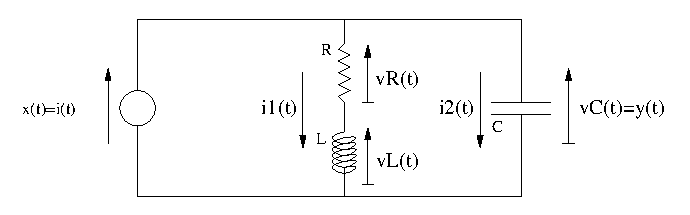
\includegraphics{circuitlrc}
\end{center}
We could find a differential equation linking the input $x(t)$ and the output $y(t)$, but it is simpler to just derive the relationship in the frequency domain.  The required quantities are
\begin{center}
  \psfrag{x(t)=i(t)}{\scriptsize $X(\omega)=I(\omega)$}
  \psfrag{vC(t)=y(t)}{\scriptsize $V_C(\omega)=Y(\omega)$}
  \psfrag{vR(t)}{\scriptsize $V_R(\omega)$}
  \psfrag{vL(t)}{\scriptsize $V_L(\omega)$}
  \psfrag{i(t)}{\scriptsize $I(\omega)$}
  \psfrag{i1(t)}{\scriptsize $I_1(\omega)$}
  \psfrag{i2(t)}{\scriptsize $I_2(\omega)$}
  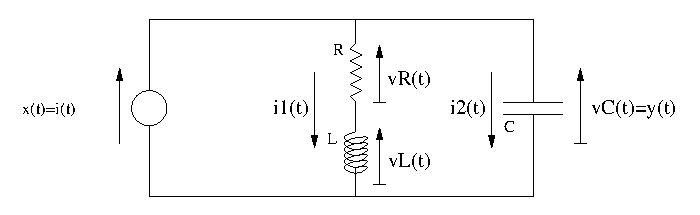
\includegraphics{circuitlrc2}
\end{center}
Now the basic voltage-current relationships for the three devices are
\begin{equation*}
  V_R(\omega) = z_R I_1(\omega), \qquad V_L(\omega) = z_L I_1(\omega), \qquad 
  V_C(\omega) = z_C I_2(\omega).
\end{equation*}
In the first branch the voltage-current relationship is
\begin{equation*}
  Y(\omega) = V_R(\omega) + V_L(\omega) = z_R I_1(\omega) + z_L I_1(\omega)
  = (z_R + z_L) I_1(\omega).
\end{equation*}
The impedances therefore add for the series combination.  Now
\begin{equation*}
  I(\omega) = I_1(\omega) + I_2(\omega) = \frac{1}{z_R + z_L} Y(\omega) + \frac{1}{z_c} Y(\omega)
  = \left( \frac{1}{z_R + z_L} + \frac{1}{z_c} \right) Y(\omega),
\end{equation*}
so the voltage-current relationship for the overall LRC combination is $Y(\omega) = z_\text{\it eff} I(\omega)$, where the effective impedance satisfies
\begin{equation*}
  \frac{1}{z_\text{\it eff}} = \frac{1}{z_R + z_L} + \frac{1}{z_c}.
\end{equation*}
This is the usual formula for combining impedances in parallel.  The overall input-output relationship satisfies
\begin{equation*}
  X(\omega) = \left( \frac{1}{R + j \omega L} + j \omega C \right) Y(\omega) 
  = \left( \frac{1 + j \omega C(R + j \omega L)}{R + j \omega L} \right) Y(\omega) 
\end{equation*}
and in terms of a system the transfer function of the circuit relating the input current to the output voltage is
\begin{equation*}
  H(\omega) = \frac{Y(\omega)}{X(\omega)} = \frac{R + j \omega L}{1 + j \omega RC + (j \omega)^2 LC}.
\end{equation*}
This transfer function is plotted below for $L=C=1$ and three different values of $R$.
\begin{center}
  \psfrag{w}{\scriptsize $\omega$}
  \psfrag{Gain GdB(w)}{\scriptsize Gain $G_{dB}(\omega)$}
  \psfrag{aG(w)}{\scriptsize $\angle G(\omega)$}
  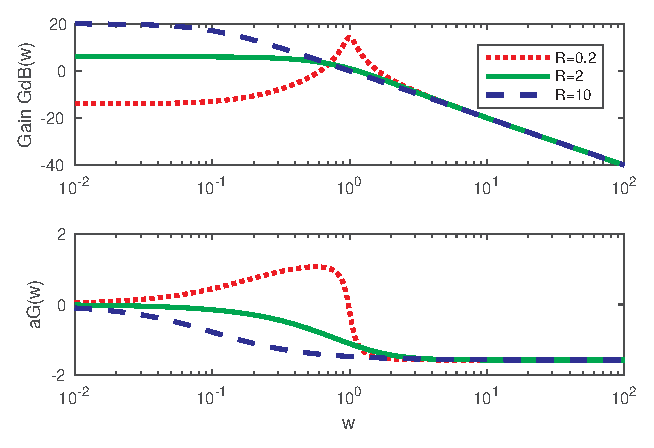
\includegraphics{rlcbpfreqresp}
\end{center}
The impulse response $h(t)$ is the inverse transform of this quantity.

Finally, note that it is possible to obtain a differential equation for the system from this transfer function.  Multiplying out gives
\begin{equation*}
  (R + j \omega L) X(\omega) = (1 + j \omega RC + (j \omega)^2 LC) Y(\omega),
\end{equation*}
and inverting gives the second-order differential equation
\begin{equation*}
  R x(t) + L \frac{d}{dt} x(t) = y(t) + RC \frac{d}{dt} y(t) + LC \frac{d^2}{dt^2} y(t).
\end{equation*}
The same expression could have been obtained using first principles in the time domain.

\subsection{General second-order response}
RLC circuit (lowpass, bandpass, highpass).


\subsection{Sampling}

All the signals considered up to this point are analog signals such as $x(t)$, expressed as a function of a time variable $t$ that can take on any real value.  While such {\em continuous-time} signals are fine up to a point, they are quite limited.  Most importantly, they don't really work in the modern world, where almost all processing is done using {\em digital} systems.  

We can sample a continuous-time signal at regular intervals to obtain a {\em discrete-time} signal:
\begin{equation*}
  x[n] = \left. x(t) \right|_{t=nT} = x(nT).
\end{equation*}
Here $n$ is an integer index, so the spacing of the samples is $T$ seconds.  The square-bracket notation $[\cdot]$ is often used instead of $(\cdot)$ to emphasise the fact that the signal is only defined for integer $n$.  It is not permitted, for example, to ask for the value of $x[3/2]$ --- it is not defined.

Let $p(t) = \sum_{n=-\infty}^{\infty} \delta(t - k T)$ be an impulse train with spacing $T$.  For a given continuous-time signal $x(t)$ we can form the sampled signal
\begin{equation*}
  x_s(t) = p(t) x(t) = \left( \sum_{n=-\infty}^{\infty} \delta(t - n T) \right) x(t)
  = \sum_{k=-\infty}^{\infty} x(nT) \delta(t - n T) = \sum_{k=-\infty}^{\infty} x[n] \delta(t - n T).
\end{equation*}
This signal $x_s(t)$ forms the link between the continuous-time domain and the discrete-time domain.  We can clearly obtain $x_s(t)$ from $x(t)$, just by using the modulation operation described, but we can also construct $x_s(t)$ from the discrete sampled signal $x[n]$ using $x_s(t) = \sum_{k=-\infty}^{\infty} x[n] \delta(t - n T)$.  In short, $x_s(t)$ contains only that information in $x(t)$ that is also present $x[n]$.  The picture in the time domain is as follows:
\begin{center}
  \psfrag{0}{\scriptsize $0$}
  \psfrag{(1)}{\scriptsize $(1)$}
  \psfrag{t}{\scriptsize $t$}
  \psfrag{T}{\scriptsize $T$}
  \psfrag{p(t)}{\scriptsize $p(t)$}
  \psfrag{x(t)}{\scriptsize $x(t)$}
  \psfrag{xs(t)}{\scriptsize $x_s(t)$}
  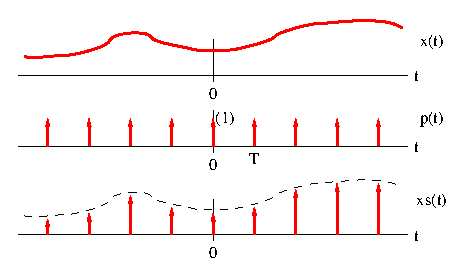
\includegraphics{sampxtime}
\end{center}

The interesting fact is that $x(t)$ can be recovered from $x_s(t)$ as long as $x(t)$ is appropriately bandlimited.  Suppose $B$ is the highest frequency present in $x(t)$, so $X(\omega) = 0$ for $|\omega| > B$.  An impulse train in time corresponds to an impulse train in frequency, so
\begin{equation*}
  P(\omega) = \omega_s \sum_{k=-\infty}^{\infty} \delta(\omega - k \omega_s)
\end{equation*}
where the sampling frequency is $\omega_s = \frac{2 \pi}{T}$.  Since multiplication in time is convolution in frequency we can find $X_s(\omega)$:
\begin{equation*}
  X_s(\omega) = \frac{1}{2\pi} P(\omega) \conv X(\omega)
  = \frac{1}{T} \sum_{k=-\infty}^{\infty} \delta(\omega - k \omega_s) \conv X(\omega)
  = \sum_{k=-\infty}^{\infty} \frac{1}{T} X(\omega - k \omega_s).
\end{equation*}
The picture in the frequency domain is as follows:
\begin{center}
  \psfrag{0}{\scriptsize $0$}
  \psfrag{w}{\scriptsize $\omega$}
  \psfrag{ws}{\scriptsize $\omega_s$}
  \psfrag{(ws)}{\scriptsize $(\frac{2\pi}{T})$}
  \psfrag{X(w)}{\scriptsize $X(\omega)$}
  \psfrag{P(w)}{\scriptsize $P(\omega)$}
  \psfrag{Xs(w)}{\scriptsize $X_s(\omega)$}
  \psfrag{A}{\scriptsize $A$}
  \psfrag{B}{\scriptsize $B$}
  \psfrag{A/T}{\scriptsize $A/T$}
  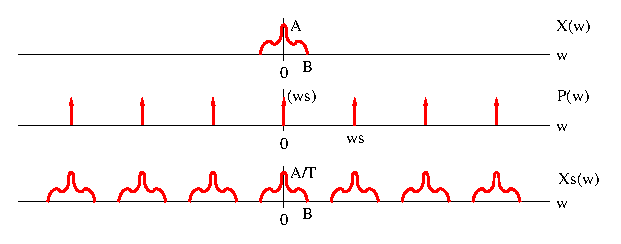
\includegraphics{sampxfreq}
\end{center}
The signal $X_s(\omega)$ can be seen to contain {\em replicas} of the signal $X(\omega)$ at integer multiples of the sampling frequency $\omega_s = \frac{2\pi}{T}$.  In the case drawn above we have $\omega_s>2B$, and the replicas are not overlapping.  Evidently we can then recover $X(\omega)$ from $X_s(\omega)$ by passing it through a filter with the following frequency response:
\begin{center}
  \psfrag{w}{\scriptsize $\omega$}
  \psfrag{ws/2}{\scriptsize $\frac{\omega_s}{2}$}
  \psfrag{Hr(w)}{\scriptsize $H_r(\omega)$}
  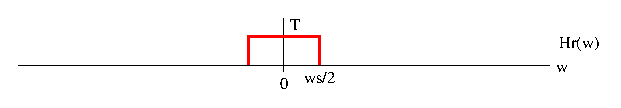
\includegraphics{sampxfilt}
\end{center}
The transfer function of this filter can be expressed as $H_r(\omega) = T P_{\omega_s}(\omega)$.

Since $X(\omega) = H_r(\omega) X_s(\omega)$ in the frequency domain, we must have $x(t) = h_r(t) \conv x_s(t)$ in time.  We can therefore reconstruct $x(t)$ from the sampled signal $x[n]$ as follows:  use the samples to form the signal
\begin{equation*}
  x_s(t) = \sum_{k=-\infty}^{\infty} x[n] \delta(t - n T),
\end{equation*}
and then put this signal through an ideal lowpass filter with impulse response
\begin{equation*}
  h_r(t) = {\cal F}^{-1} \{H_r(\omega)\} = \text{sinc} \left(\frac{t}{T}\right)
\end{equation*}
to recover the original $x(t)$.  Equivalently we can write the reconstruction formula as
\begin{equation*}
  x(t) = x_s(t) \conv h_r(t) = \sum_{k=-\infty}^{\infty} x[n] h_r(t - n T) = \sum_{k=-\infty}^{\infty} x[n] \text{sinc}\left(\frac{1}{T} (t - n T) \right).
\end{equation*}

The reconstruction process works as long as the spectral replicas in $X_s(\omega)$ are not overlapping.  Note, though, that these replicas occur at spacings $\omega_s = \frac{2\pi}{T}$.  Thus if we choose $T$ such that $\omega_s \geq 2B$ is satisfied then the signal $x(t)$ can be reconstructed from $x[n]$.  The signal must be sampled at {\em twice its highest frequency} for this to be possible.  This is called the {\em Nyquist} sampling criterion, and $\omega_s = 2B$ is called the {\em Nyquist sampling rate}.

In the case shown above the sampling frequency $\omega_s$ is bigger than it needs to be for perfect reconstruction to be possible, since the replicas are far from overlapping.  Equivalently, the sampling period $T$ is smaller than it has to be --- we have more samples than are required.    The signal is said to be {\em over-sampled}, and this is a good thing.

If we choose $\omega_s = 2B$ then the signal $x(t)$ is {\em critically sampled}.  The frequency plots then look like this:
\begin{center}
  \psfrag{0}{\scriptsize $0$}
  \psfrag{w}{\scriptsize $\omega$}
  \psfrag{ws}{\scriptsize $\omega_s$}
  \psfrag{(ws)}{\scriptsize $(\frac{2\pi}{T})$}
  \psfrag{X(w)}{\scriptsize $X(\omega)$}
  \psfrag{P(w)}{\scriptsize $P(\omega)$}
  \psfrag{Xs(w)}{\scriptsize $X_s(\omega)$}
  \psfrag{A}{\scriptsize $A$}
  \psfrag{B}{\scriptsize $B$}
  \psfrag{A/T}{\scriptsize $A/T$}
  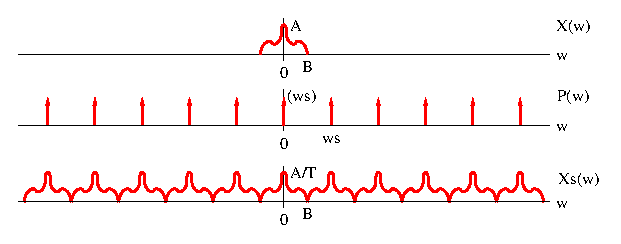
\includegraphics{sampxfreq2}
\end{center}
The signal $x(t)$ can {\em just} be reconstructed from the samples $x[n]$, although to do this we do need a perfect reconstruction filter.

If we sample at a spacing larger than the spacing for this critical frequency --- in other words, if we take too few samples --- then the spectral replicas will overlap and we say that {\em aliasing} has occurred.  It is important to note that the signal $X_s(\omega)$ contains the {\em sum} of all the shifted replicas:  if they overlap then it is impossible to recover each individual replica, in the same way that it is impossible to determine $x$ and $y$ given that $x+y = 10$.  In this case the signal has been destroyed by the discretisation process:  there is no way to recover $x(t)$ from $x[n]$.  The signal has been {\em under-sampled}, aliasing has occurred, and $x(t)$ has been lost.

\end{document}
